%%\usetikzlibrary{arrows,shapes,automata, positioning}
\usetikzlibrary{arrows,shapes,automata}

%% \begin{figure}[ht]
%% \begin{subfigure}[t]{.4\textwidth}
%% \centering
%% \small
%% \begin{tikzpicture}[->,>=stealth',shorten >=1pt,auto,node distance=3cm,
%%                     thick,initial text={},initial above]
%%   \tikzstyle{every state}=[fill=white,draw,ellipse,text=black]
%%   \node[initial,state] (A)                    {$\mathsf{Init}$};
%%   \node[state]         (B) [below right of=A] {$\mathsf{Written\ t}$};
%%   \node[state]         (D) [below left of=A] {$\mathsf{Clean\ t}$};
%%   \node[state]         (C) [below left of=B] {$\mathsf{Dirty\ t}$};
 
%%   \path (A) edge [bend left]  node {$\act{register}(p,v)$} (B)
%%         (B) edge [bend left]  node {$\act{check}(p,true)$} (C)
%%             edge              node {$\act{check}(p,false)$} (D)
%%         (C) edge [bend left]  node {$\act{forward}(p)$}(D)
%%         (D) edge [bend left]  node {$\act{exit}()$} (A);
%% \end{tikzpicture}
%% \caption{\label{fig:sts:writer} Write STS on $\wstate{p}$}
%% \end{subfigure}%
%% \begin{subfigure}[t]{.6\textwidth}
%% \centering
%% \small
%% \begin{tikzpicture}[->,>=stealth',shorten >=1pt,auto,node distance=2.2cm,
%%                     thick,initial text={},]
%%   \tikzstyle{every state}=[fill=white,draw,ellipse,text=black]
%%   \node[initial,state] (A)                     {$(\FF,\FF,\FF)$};
%%   \node[state]         (B)  [above right of=A] {$(\TT,\FF,\FF)$};
%%   \node[state]         (C1) [above right of=B] {$(\TT,\TT,\FF)$};
%%   \node[state]         (C2) [below right of=B] {$(\TT,\FF,\TT)$};
%%   \node[state]         (D)  [right=2.5 cm of B]  {$(\TT,\TT,\TT)$};
%%   \node[state]         (E)  [below right=0.5cm and 0.cm of C2]
%%                               {$(\FF,\TT,\TT)$};
%%   \path (A)  edge [bend left]   node {$\act{set}(\TT)$} (B)
%%         (B)  edge [bend left]   node {$\act{clear}(\mathtt{x})$} (C1)
%%              edge [bend right]  node {$\act{clear}(\mathtt{y})$} (C2)
%%         (C1) edge [bend left]   node {$\act{clear}(\mathtt{y})$} (D)
%%         (C2) edge [bend right]  node {$\act{clear}(\mathtt{x})$} (D)
%%         (D)  edge [bend left]   node {$\act{set}(\FF)$} (E)
%%         (E)  edge [bend left]   node {$\act{relink}(rx,ry)$} (A);
%% \end{tikzpicture}
%% \caption{\label{fig:sts:scanner} Scan STS on $\wstate{S}$}
%% \end{subfigure}
%%  \caption{\label{fig:sts} The State Transition System described by auxiliary code}
%% \end{figure}

% I don't need the scanner protocol at all
\begin{wrapfigure}[15]{r}[0pt]{0.5\textwidth} 
\centering
\small
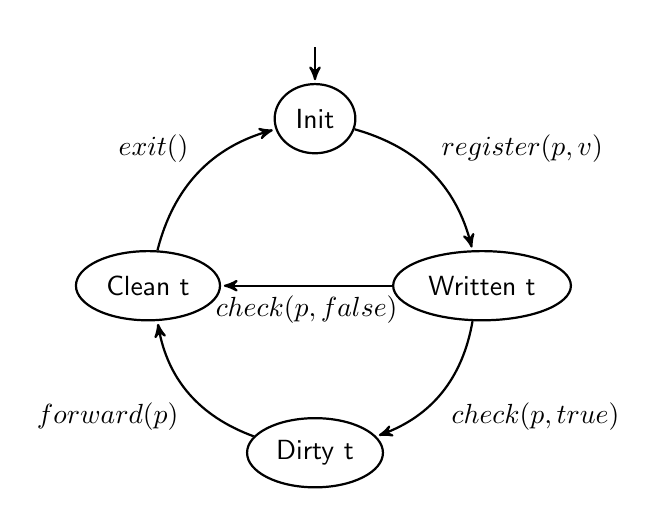
\begin{tikzpicture}[->,>=stealth',shorten >=1pt,auto,node distance=3cm,
                    thick,initial text={},initial above]
  \tikzstyle{every state}=[fill=white,draw,ellipse,text=black]
  \node[initial,state] (A)                    {$\mathsf{Init}$};
  \node[state]         (B) [below right of=A] {$\mathsf{Written\ t}$};
  \node[state]         (D) [below left of=A] {$\mathsf{Clean\ t}$};
  \node[state]         (C) [below left of=B] {$\mathsf{Dirty\ t}$};
 
  \path (A) edge [bend left]  node {$\act{register}(p,v)$} (B)
        (B) edge [bend left]  node {$\act{check}(p,true)$} (C)
            edge              node {$\act{check}(p,false)$} (D)
        (C) edge [bend left]  node {$\act{forward}(p)$}(D)
        (D) edge [bend left]  node {$\act{exit}()$} (A);
\end{tikzpicture}
\caption{\label{fig:sts} Write STS on $\wstate{p}$}
\end{wrapfigure}
